\subsection{Annotation Pipeline Components and theirs
Configurations}\label{annotation-pipeline-components-and-theirs-configurations}

The deidentification tool was designed to be relatively flexible to
accommodate various needs.

\subsection{Data Input}\label{data-input}

More details on the configuration of the report input data source.

\subsubsection{DB Configuration}\label{db-configuration}

Configuration parameters to load reports from a database are stored in a
text file (properties file) with the following attributes
(example config in Section~\ref{adapt-database-configuration}):

\begin{itemize}
\tightlist
\item
  \texttt{jdbc\_url}: the URL to connect to the database,
  \href{https://docs.oracle.com/javase/tutorial/jdbc/basics/connecting.html}{see
  also}
\item
  \texttt{user}: the database user name
\item
  \texttt{password}: the password
\item
  \texttt{query}: a ``SELECT'' SQL query. Can be anything (e.g.~joining
  data from several tables, a view \ldots) as long as certain columns
  are present
\item
  \texttt{json\_field\_name}: the column name in the above SQL query
  denoting the JSON content of a report
\item
  \texttt{reportid\_field\_name}: the column name denoting the reportid
  of a report in the SQL query
\item
  \texttt{report\_type\_id}: the column name in the above query denoting
  the report type (``FCODE'') of a report. This is mainly used to select
  certain types of reports.
\item
  \texttt{date\_field\_name}: the column name in the above query
  denoting the creation date of a report (optional).
\end{itemize}

In case reports should be written back to a database after substitution:
* \texttt{dest\_table}: table name to write into *
\texttt{dest\_columns}: the names of the columns to write back. These
should be a subset of the columns in the above SELECT SQL query (could
also be all of them)

\paragraph{Report Filtering}\label{report-filtering}

\subparagraph{Document Type Filter}\label{document-type-filter}

Depending on the project, only certain document types (``FCODE'') might
be relevant. These could be filtered out in the SQL query or also using
a simple text file which can be passed to the \texttt{annotate} or
\texttt{import} command using the \texttt{-\/-doc-type-filter} option.

The file contains one row per document type and at least one column
(seperated by `,'), where the first column denotes the document type
name. There can be more columns (for example human readable
description), which are ignored by the application.

\subparagraph{Document ID Filter}\label{document-id-filter}

Similar to document type filters, one can specify to load only documents
having a specific ID. This can be done by passing a file path using the
\texttt{-\/-doc-id-filter} option.

Columns: * report id

\subsection{Annotation Pipeline}\label{annotation-pipeline}

Quite a few aspects of the annotation pipeline can be parameterized. In
this section, more details about various annotation steps and their
configuration.

\subsubsection{Pipeline Configuration
File}\label{pipeline-configuration-file}

Many pipeline steps can be parametrized by specific configuration files
or other parameters. The parametrization happens via a configuration
file setting all relevant parameters for the annotation pipeline. You
can pass the path of the file to the \texttt{annotate} command using
\texttt{-c}. The syntax of the file follows the
\href{https://github.com/lightbend/config}{HOCON format}, see the
\href{https://github.com/ratschlab/medical-reports-deidentification/blob/main/configs/kisim-usz/kisim_usz.conf}{configuration of the USZ
pipeline as example}

Configurations relevant to the pipeline are grouped together into the
\texttt{pipeline} `section'.

\subsubsection{Lexica (Dictionaries,
Gazetteers)}\label{lexica-dictionaries-gazetteers}

The \texttt{pipeline.gazetteer} option should point to a GATE gazetteer
file definition (\texttt{*.def}). This text file contains an entry for
each dictionary file with the (relative) path and the annotation type. A
dictionary file is simply a text file with one or more token per line.
More details in the
\href{https://gate.ac.uk/sale/tao/splitch6.html\#x9-1270006.3}{GATE
Documentation}

The annotation pipeline also uses a second category of gazetteers
specified in \texttt{pipeline.suffixGazeteer} not matching entire tokens
but suffixes. This is useful for rules based on word endings, for
example to recognize surnames (``-mann'', ``-oulos'', ``-elli'') and
medical terms (``-karzinom'', ``-suffizienz'', ``-beschwerden'').

\subsubsection{Specific JAPE Rules}\label{specific-jape-rules}

There is a generic set of JAPE rules shipped with the application.
Typically, these rules cannot cover special cases appearing in a given
organization. This can be done using a separate rule set.

Specific rules can be added via the \texttt{pipeline.specificTransducer}
option pointing to a \texttt{*.jape} file. This file would contain a
list of different phases, where every phase is a separate
\texttt{*.jape} file. These files would then contain the actual JAPE
rules. See also the
\href{https://gate.ac.uk/sale/tao/splitch8.html\#x12-2310008.5}{Gate
Documentation}.

\subsubsection{Report Structure}\label{report-structure}

If available, the structure of input documents can be exploited during
the annotation (and in principle also during substitution). That is,
prior knowledge about the document can be added.

In case of JSON, the structure elements would be field names and nested
objects. A JSON document can then be seen as a tree where the leaves
contain the actual report text fragments.

\begin{figure}
\centering
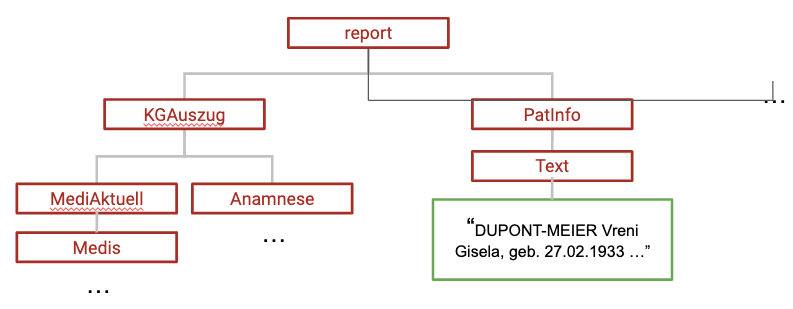
\includegraphics[width=\textwidth]{figs/report_structure.png}
\caption{simple report structure}
\end{figure}

\paragraph{Paths in Field Tree}\label{paths-in-field-tree}

In the various configuration files related to annotations, paths in the
``field tree'' can be used to denote certain parts of the document
(similar to XPath for XML documents).

A \textbf{path} can consist of the following elements: * field name: can
be a
\href{https://docs.oracle.com/javase/8/docs/api/java/util/regex/Pattern.html}{regular
expression accepted by Java} * `/' denoting that the nodes must appear
consecutively, e.g.~\texttt{field\_a/field\_c} matches only
``field\_a/field\_c'' but not ``field\_a/field\_b/field\_c'' . * `//'
denoting that the nodes don't need to be necessarily consecutive, e.g.
\texttt{field\_a/field\_c} would match both ``field\_a/field\_c'' and
``field\_a/field\_b/field\_c''

Note, that paths are case-sensitive.

Examples:
Simple field names which can appear anywhere in the tree: *
\texttt{Id} * \texttt{ID} * some regular expression
\texttt{{[}\textbackslash{}\textbackslash{}p\{IsAlphabetic\}{]}*VisDat}
(``\\p'' is used to match unicode characters). * Field names with some
constraints regarding the parent. For instance, to match \texttt{Text}
fields only when it is a child of \texttt{PatInfo}, you can use
\texttt{//PatInfo//Text}, which would match
e.g.~``/report/PatInfo/some\_element/Text'' * Field constraints
``anchored'' from the top: \texttt{/NOTE} would match a field ``NOTE''
directly under the root of a tree, but not ``/PatientInfo/NOTE''.

\paragraph{Structured Annotations}\label{structured-annotations}

The ``structured annotation step'' allows annotating entire text fields.
For instance, if you know that a certain field contains the name of a
person, then an annotation can be performed at that level.

This step can be parametrized with a configuration file passed in
\texttt{pipeline.structuredFieldMapping} in the pipeline configuration.

Columns in the config file (separated by ``;''): * Path * Annotation
type (e.g.~\texttt{Name}, \texttt{Date} etc) * Features (properties) of
the annotation . Features are separated by ``,'' where key and values
are separated by ``=''

Example: \texttt{//Personalien//Name;\ Name;\ type=patient}

All leaves with \texttt{Name} having \texttt{Personalien} as a parent
somewhere are annotated with \texttt{Name} and having the \texttt{type}
property set to \texttt{patient}.

\paragraph{Field Normalization (Field Annotation
Mapping)}\label{field-normalization-field-annotation-mapping}

Sometimes, we can not blindly annotate an entire field, but need to
apply a JAPE rule on it. For example, signatures could have a structure
like ``ABCD, 20.10.2018'' where ``ABCD'' is the shorthand for a doctor.
Since there are many fields with similar or identical structure, but
different paths the fields can get renamed to a common name. A JAPE rule
processing the pattern would then refer to that common name.

This step can be parametrized with a configuration file passed in
\texttt{pipeline.annotationMapping} in the pipeline configuration.
Columns (separated by ``;''): * Path * New field name

Example: \texttt{//Patient/Alter/Val;\ AgeField}

A field \texttt{Val} with immediate ancestors \texttt{Alter} and
\texttt{Patient} gets named an \texttt{AgeField}. Now a JAPE rule only
working on \texttt{AgeField}s, could for example annotate any number in
there as an age.

\paragraph{Annotation Blacklist}\label{annotation-blacklist}

For some fields we can exclude a priori certain annotations. An example
could be a field containing computer generated identifiers like
\texttt{9b02d92c-c16e-4d71-2019-280237bb8cb5} where a JAPE rule may
erroneously pick up a date (for example ``2019'' in the example). A
blacklisting step would remove such annotations.

This step can be parametrized with a configuration file passed in
\texttt{pipeline.annotationBlacklist} in the pipeline configuration.

Columns (seperated by ``;''): * Path * Comma separated annotation types
which should \emph{not} appear within elements denoted in path

Example: \texttt{//DiagnList//CodeList//Version;\ Date}

The \texttt{Version} field having \texttt{CodeList} and
\texttt{DiagnList} as parents should not contain \texttt{Date}
annotations.

\subsubsection{Context Annotations}\label{context-annotations}

There are some JAPE rules which only get triggered if tokens appear in a
specific language context. This can be useful to disambiguate between
e.g.~surnames and professions or between the profession of a patient vs
the role of staff.

The context can be given by a field (using
\hyperref[field-normalization-field-annotation-mapping]{Annotation Mappings}) or by using
\textbf{context annotations}. They can be added around trigger tokens.
For instance, text in the vicinity of \texttt{Sohn} (son) may contain
his name or information about his profession. Therefore,
\texttt{NameContext} and \texttt{OccupationContext} context annotations
are added to the document, spanning the e.g.~5 tokens before
\texttt{Sohn} and 5 tokens after. Later on, if within these context
annotations e.g.~an isolated first name appears, it can be annotated as
\texttt{Name} since we assume it is a context where names can occur
(otherwise we wouldn't annotate it, as there is not enough evidence).
Context annotations are performed in early stages of the pipeline, s.t.
they can be referred to in JAPE rules later on.

These context triggers can be configured in a config file whose path has
to be provided in \texttt{pipeline.contextTriggerConfig} in the pipeline
configuration.

Columns (separated by ``;''): * Context token (no spaces) * Name of the
context (e.g.~\texttt{NameContext}) * start of the context annotation in
number of tokens before the trigger token * end of the context
annotation in number of tokens after the trigger token

Examples: * \texttt{Sohn;NameContext;5;5} *
\texttt{Partner;OccupationContext;5;5}

\subsection{Test Suite}\label{test-suite}

A small testing framework was developed to test the annotation behavior
of the pipeline in a fast and isolated way. That is, small test cases
can be defined consisting of a phrase and the annotations the pipeline
is expected to produce. This allows for test driven development/tuning
of the annotation pipeline.

\subsubsection{Test Cases Specification}\label{test-cases-specification}

The testcases are described in a textfile. The first line of the text
file contains the annotation types the pipeline is tested against as
well as the context fields. The context fields annotations are used to
test rules based on the document structure. The lists for annotation
types and context fields are seperated by \texttt{;} and the entries in
lists by \texttt{,}.

Then testcases follow, one per line. Manual annotations and fields are
added using XML-tags. Comments using `\#' are allowed either to comment
entire lines are the remainder of a line. Commented parts are ignored.
There may be empty lines for making the file a bit more readable. If new
lines are needed to test a specific situation, this can simply be done
using \texttt{\textbackslash{}n}.

Following an example with 3 test cases:

\begin{verbatim}
Name; FieldWithSignature

Der Patient <Name>Luigi D'Ambrosio</Name> wurde...

<FieldWithSignature>20.01.2018 / <Name>AMUSTER</Name> </FieldWithSignature>
20.01.2018 / AMUSTER # don't expect name annotation in arbitrary fields
\end{verbatim}

In this example, the annotation of \texttt{Name} is tested. The
\texttt{\textless{}Name\textgreater{}} tags are removed before the test
case is passed through the pipeline. Then, the \texttt{Name} annotations
of the pipeline output are checked whether they indeed contain
\texttt{Name} annotations at the same place, and only there. If this is
the case, the test passes, otherwise it fails with an appropriate
message.

The second test case tests a context specific rule, i.e.~the rule is
only applied within fields \texttt{FieldWithSignature} (In the USZ
pipeline, \texttt{FieldWithSignature} annotation is added the annotation
mapping step, see above) The third test case is just to see, if the
previous rule is not triggered outside the required context. Or said
differently, we expect \texttt{AMUSTER} not to be annotated,
i.e.~annotating it would be wrong.

In some existing tests there is also the \texttt{OUTOFVOC} token. It
stands for ``out of vocabulary'' and makes it explicit, that the rule
should rely exclusively on structure, and not be based on entries in the
dictionary.

\subparagraph{Running Tests}\label{running-tests}

A test suite can be run using the \texttt{test} command from the
\texttt{DeidMain} entry point:

\begin{verbatim}
$DEID_CMD test [pipeline configuration file] [testcase directory]
\end{verbatim}

It commands needs a path to a pipeline configuration file
(e.g.~\texttt{configs/kisim-usz/kisim\_usz.conf}) and a directory with
testcases (e.g.~\texttt{configs/kisim-usz/testcases/}). Every
\texttt{*.txt} in that directory is assumed to contain test cases.

The generic rules shipped with the tool are tested using the same
mechanism. They are run as unit tests for the tool itself. The test
cases can be found in the directory
\texttt{deidentifier-pipeline/src/test/resources/pipeline\_testcases}
You normally don't need to modify these tests while tuning the pipeline,
but you may consider them a source of useful examples.
